%%%%%%%%%%%%%%%%%%%%%%%%%%%%%%%%%%%%%%%%%%%%%%%%%%%%%%%%%%%%%%%%%%% 
%                                                                 %
%                            CHAPTER                              %
%                                                                 %
%%%%%%%%%%%%%%%%%%%%%%%%%%%%%%%%%%%%%%%%%%%%%%%%%%%%%%%%%%%%%%%%%%% 

\chapter{Thesis details}

\textbf{Title: } Inversion: from knowledge graphs to raw data

\textbf{Subject: } 
\begin{itemize}
	\item \textbf{RQ1: } How can we leverage RML to construct raw data from heterogeneous data.
	\item \textbf{RQ2: } How can we extend an existing system like RML or create a new system to construct raw data from knowledge graphs.
\end{itemize}

\textbf{Description: } Knowledge graphs are gaining traction nowadays and more and more companies use them, such as Amazon, Bosch, IKEA, Facebook, Google, LinkedIn, SIEMENS, Zalando, etc. Most knowledge graphs are nowadays constructed from other heterogeneous data sources, such as tables in relational databases, data in XML files or in JSON format derived from a Web API. While the construction of knowledge graphs from heterogeneous data was theoroughly investigated so far, the inverse, namely constructing raw data from knowledge graphs is not explored so far.

\textbf{Company: } internal research group EAVISE, CAMPUS DE NAYER

\textbf{University promotor: } Anastasia Dimou

\textbf{Planning: } see gantt chart in figure \ref{fig:gantt_chart}



\begin{figure}[htbp]
	\makebox[\textwidth]{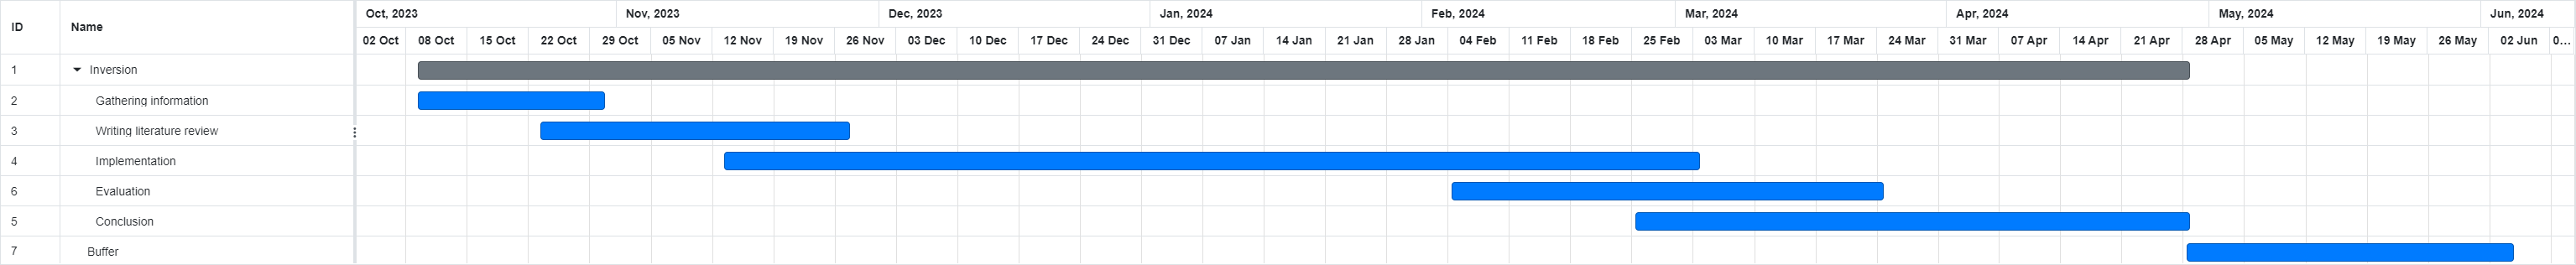
\includegraphics[width=\paperwidth]{fig/startup_report/gantt.png}}
	\caption{Gantt chart}
	\label{fig:gantt_chart}
  \end{figure}
